\documentclass[aspectratio=169]{beamer}
\usetheme{Madrid}
\usecolortheme{default}

% Packages
\usepackage{graphicx}
\usepackage{listings}
\usepackage{booktabs}
\usepackage{tikz}
\usetikzlibrary{shapes,arrows,positioning}
\lstset{
  language=C++,
  backgroundcolor=\color{codebg},
  basicstyle=\tiny\ttfamily,
  keywordstyle=\color{blue},
  commentstyle=\color{codegreen},
  stringstyle=\color{red},
  breaklines=true,
  frame=single,
  numbers=left,
  numberstyle=\tiny\color{codegray}
}


% Custom colors
\definecolor{codebg}{rgb}{0.95,0.95,0.95}
\definecolor{codegreen}{rgb}{0,0.6,0}
\definecolor{codegray}{rgb}{0.5,0.5,0.5}

% Listings style
\lstset{
    backgroundcolor=\color{codebg},
    basicstyle=\tiny\ttfamily,
    keywordstyle=\color{blue},
    commentstyle=\color{codegreen},
    stringstyle=\color{red},
    breaklines=true,
    frame=single,
    numbers=left,
    numberstyle=\tiny\color{codegray}
}

\title{Huxley: Embedded Chat Server}
\subtitle{Design Specification}
\author{System Architecture \& Design}
\date{\today}

\begin{document}

\frame{\titlepage}

% Table of Contents
\begin{frame}{Outline}
    \tableofcontents
\end{frame}

%===========================================
\section{Introduction}
%===========================================

\begin{frame}{System Overview}
    \begin{columns}
        \column{0.5\textwidth}
        \textbf{Huxley Chat Server}
        \begin{itemize}
            \item Embedded messaging system
            \item Raspberry Pi 4 platform
            \item Client-server architecture
            \item Multi-threaded design
            \item 25+ concurrent users
        \end{itemize}
        
        \column{0.5\textwidth}
        \textbf{Key Features}
        \begin{itemize}
            \item Secure authentication (Argon2id)
            \item Message encryption (XSalsa20-Poly1305)
            \item Offline message queuing
            \item Real-time delivery
            \item RGB LED status indicator
        \end{itemize}
    \end{columns}
\end{frame}

\begin{frame}{Design Philosophy}
    \begin{block}{Defense in Depth}
        Multiple independent security layers: password hashing, SQL injection prevention, message encryption, audit logging
    \end{block}
    
    \begin{block}{SOLID Principles}
        \begin{itemize}
            \item Single Responsibility: Each class has one well-defined purpose
            \item Dependency Inversion: Components depend on abstractions
            \item Loose Coupling: Clean separation between I/O, business logic, and persistence
        \end{itemize}
    \end{block}
\end{frame}

%===========================================
\section{Hardware Specification}
%===========================================

\begin{frame}{Hardware Components}
    \begin{columns}
        \column{0.6\textwidth}
        \textbf{Raspberry Pi 4 Model B}
        \begin{itemize}
            \item 4GB RAM (supports concurrent connections)
            \item Quad-core ARM Cortex-A72 @ 1.5GHz
            \item GPIO pins for LED control
            \item Gigabit Ethernet
            \item 5V 3A USB-C power supply
        \end{itemize}
        
        \vspace{0.3cm}
        \textbf{RGB LED Status Indicator}
        \begin{itemize}
            \item Green: System idle/ready
            \item Yellow: Processing requests
            \item Red: Error condition
            \item GPIO pins: 17, 27, 22 (R/G/B)
            \item Current-limiting resistors: 220Ω-470Ω
        \end{itemize}
        
        \column{0.4\textwidth}
        \begin{center}
            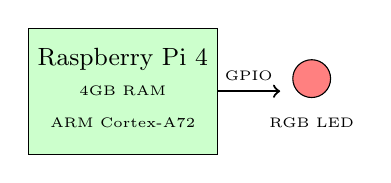
\begin{tikzpicture}[scale=0.8]
                % Raspberry Pi
                \draw[fill=green!20] (0,0) rectangle (3,2);
                \node at (1.5,1.5) {\small Raspberry Pi 4};
                \node at (1.5,1) {\tiny 4GB RAM};
                \node at (1.5,0.5) {\tiny ARM Cortex-A72};
                
                % GPIO connection
                \draw[thick,->] (3,1) -- (4,1) node[midway,above] {\tiny GPIO};
                
                % LED
                \draw[fill=red!50] (4.5,1.2) circle (0.3);
                \node at (4.5,0.5) {\tiny RGB LED};
            \end{tikzpicture}
        \end{center}
    \end{columns}
\end{frame}

%===========================================
\section{Software Architecture}
%===========================================

\begin{frame}{Software Stack}
    \begin{columns}
        \column{0.5\textwidth}
        \textbf{Development Tools}
        \begin{itemize}
            \item Buildroot (embedded Linux)
            \item GCC ARM cross-compiler
            \item VS Code
        \end{itemize}
        
        \vspace{0.3cm}
        \textbf{Core Libraries}
        \begin{itemize}
            \item SQLite 3.46.0 (database)
            \item libsodium 1.0.20 (crypto)
            \item PThreads (concurrency)
        \end{itemize}
        
        \column{0.5\textwidth}
        \begin{block}{SQLite Features}
            \begin{itemize}
                \item WAL mode (concurrent reads)
                \item Prepared statements
                \item Zero administration
                \item ACID guarantees
            \end{itemize}
        \end{block}
        
        \begin{block}{libsodium Features}
            \begin{itemize}
                \item Argon2id password hashing
                \item XSalsa20+Poly1305 encryption
                \item Constant-time operations
                \item Automatic key derivation
            \end{itemize}
        \end{block}
    \end{columns}
\end{frame}

%===========================================
\section{Database Design}
%===========================================

\begin{frame}[fragile]{Database Schema}
    \begin{columns}
        \column{0.5\textwidth}
        \textbf{Users Table}
\begin{lstlisting}[language=SQL]
CREATE TABLE users (
  id INTEGER PRIMARY KEY,
  username TEXT UNIQUE NOT NULL,
  password_hash TEXT NOT NULL,
  created_at TIMESTAMP DEFAULT 
    CURRENT_TIMESTAMP
);
CREATE INDEX idx_username 
  ON users(username);
\end{lstlisting}

        \vspace{0.2cm}
        \textbf{Messages Table}
\begin{lstlisting}[language=SQL]
CREATE TABLE messages (
  id INTEGER PRIMARY KEY,
  sender_id INTEGER NOT NULL,
  recipient_id INTEGER NOT NULL,
  content_encrypted BLOB NOT NULL,
  timestamp TIMESTAMP,
  delivered BOOLEAN DEFAULT 0,
  FOREIGN KEY (sender_id) 
    REFERENCES users(id),
  FOREIGN KEY (recipient_id)
    REFERENCES users(id)
);
\end{lstlisting}
        
        \column{0.5\textwidth}
        \textbf{Logs Table}
\begin{lstlisting}[language=SQL]
CREATE TABLE logs (
  id INTEGER PRIMARY KEY,
  message TEXT NOT NULL,
  timestamp TIMESTAMP DEFAULT
    CURRENT_TIMESTAMP
);
CREATE INDEX idx_log_timestamp
  ON logs(timestamp DESC);
\end{lstlisting}

        \vspace{0.3cm}
        \textbf{WAL Mode Configuration}
\begin{lstlisting}[language=SQL]
PRAGMA journal_mode=WAL;
PRAGMA synchronous=NORMAL;
\end{lstlisting}

        \vspace{0.2cm}
        \begin{alertblock}{Why WAL?}
            Enables 25 concurrent reads during writes - critical for real-time messaging
        \end{alertblock}
    \end{columns}
\end{frame}

\begin{frame}{Indexing Strategy}
    \begin{block}{Performance Optimization}
        \begin{itemize}
            \item \texttt{idx\_username}: O(log n) user lookup during authentication
            \item \texttt{idx\_recipient\_delivered}: Fast queued message retrieval
            \item \texttt{idx\_sender\_timestamp}: Efficient message history queries
            \item \texttt{idx\_log\_timestamp}: Latest log entry access
        \end{itemize}
    \end{block}
    
    \vspace{0.3cm}
    \begin{columns}
        \column{0.5\textwidth}
        \textbf{Without Index}
        \begin{itemize}
            \item Full table scan: O(n)
            \item Slow with 1000+ users
            \item Poor concurrency
        \end{itemize}
        
        \column{0.5\textwidth}
        \textbf{With Index}
        \begin{itemize}
            \item B-tree lookup: O(log n)
            \item Sub-millisecond queries
            \item Scales to 10,000+ users
        \end{itemize}
    \end{columns}
\end{frame}

%===========================================
\section{Security Architecture}
%===========================================

\begin{frame}[fragile]{Password Hashing: Argon2id}
    \begin{columns}
        \column{0.5\textwidth}
        \textbf{Threat Model}
        \begin{itemize}
            \item Attacker obtains database file
            \item Goal: recover user passwords
            \item Defense: Memory-hard hashing
        \end{itemize}
        
        \vspace{0.3cm}
        \textbf{Argon2id Properties}
        \begin{itemize}
            \item 128-bit unique salt per password
            \item 64 MB RAM per hash
            \item 2 CPU iterations
            \item Defeats rainbow tables
            \item Defeats GPU brute force
        \end{itemize}
        
        \column{0.5\textwidth}
\begin{lstlisting}[language=C++]
// Hash password
HashPassword(pw):
  salt = random(16 bytes)
  hash = argon2id(
    password=pw,
    salt=salt,
    mem=64MB,
    iter=2
  )
  return "$argon2id$v=19$" +
    "m=65536,t=2,p=1$" +
    base64(salt) + "$" +
    base64(hash)

// Verify password
VerifyPassword(pw, stored):
  extract salt, params
  derived = argon2id(pw, salt)
  return constant_time_compare(
    derived, stored
  )
\end{lstlisting}
    \end{columns}
\end{frame}

\begin{frame}[fragile]{SQL Injection Prevention}
    \begin{columns}
        \column{0.5\textwidth}
        \textbf{Threat Scenario}
        \begin{itemize}
            \item Attacker sends:\\
            \texttt{username = "admin'; DROP TABLE users; --"}
            \item Goal: Execute malicious SQL
        \end{itemize}
        
        \vspace{0.3cm}
        \textbf{Vulnerable Code (NEVER USE)}
\begin{lstlisting}[language=C++]
string sql = 
  "SELECT * FROM users " +
  "WHERE username='" + 
  username + "';";
sqlite3_exec(db, sql.c_str());
// EXPLOITABLE!
\end{lstlisting}
        
        \column{0.5\textwidth}
        \textbf{Secure Implementation}
\begin{lstlisting}[language=C++]
// Use prepared statements
sqlite3_stmt* stmt;
sqlite3_prepare_v2(db,
  "SELECT * FROM users "
  "WHERE username=?",
  -1, &stmt, NULL
);

// Bind parameter as literal
sqlite3_bind_text(
  stmt, 1, 
  username.c_str(),
  -1, SQLITE_TRANSIENT
);

// Execute safely
sqlite3_step(stmt);
sqlite3_finalize(stmt);
\end{lstlisting}

        \begin{alertblock}{Result}
            SQL structure is fixed - input cannot alter query logic
        \end{alertblock}
    \end{columns}
\end{frame}

\begin{frame}[fragile]{Message Encryption}
    \begin{columns}
        \column{0.5\textwidth}
        \textbf{Encryption Algorithm}
        \begin{itemize}
            \item XSalsa20 stream cipher
            \item Poly1305 MAC (integrity)
            \item 256-bit master key
            \item 24-byte random nonces
        \end{itemize}
        
        \vspace{0.3cm}
        \textbf{Key Management}
        \begin{itemize}
            \item Single master key
            \item Stored: \texttt{/etc/huxley/master.key}
            \item Permissions: \texttt{chmod 400}
            \item Generated on first boot
        \end{itemize}
        
        \column{0.5\textwidth}
\begin{lstlisting}[language=C++]
// Encrypt message
EncryptMessage(plaintext):
  nonce = random(24 bytes)
  ciphertext = 
    crypto_secretbox(
      plaintext,
      nonce,
      masterKey
    )
  return nonce || ciphertext

// Decrypt message
DecryptMessage(encrypted):
  nonce = encrypted[0:24]
  ciphertext = encrypted[24:]
  plaintext = 
    crypto_secretbox_open(
      ciphertext,
      nonce,
      masterKey
    )
  if MAC_invalid:
    reject message
  return plaintext
\end{lstlisting}
    \end{columns}
    
    \vspace{0.2cm}
    \textbf{Storage Format:} [24-byte nonce][ciphertext + 16-byte MAC] = 40 bytes overhead
\end{frame}

\begin{frame}{Security Properties}
    \begin{block}{Password Security}
        \begin{itemize}
            \item Testing 1 million passwords takes $\sim$30 minutes on RPi4
            \item Unique salt prevents rainbow table attacks
            \item Configurable work factor adapts to hardware improvements
        \end{itemize}
    \end{block}
    
    \begin{block}{Message Security}
        \begin{itemize}
            \item \textbf{Confidentiality:} Attacker with database cannot read messages
            \item \textbf{Integrity:} Modified ciphertexts fail MAC verification
            \item \textbf{Replay Protection:} Unique nonces prevent message reuse
            \item \textbf{Performance:} $\sim$1 microsecond per message
        \end{itemize}
    \end{block}
    
    \begin{block}{Activity Logging}
        Every security event logged: logins, failed attempts, message sends, disconnects
    \end{block}
\end{frame}

%===========================================
\section{Class Architecture}
%===========================================

\begin{frame}{System Architecture Overview}
    \begin{center}
        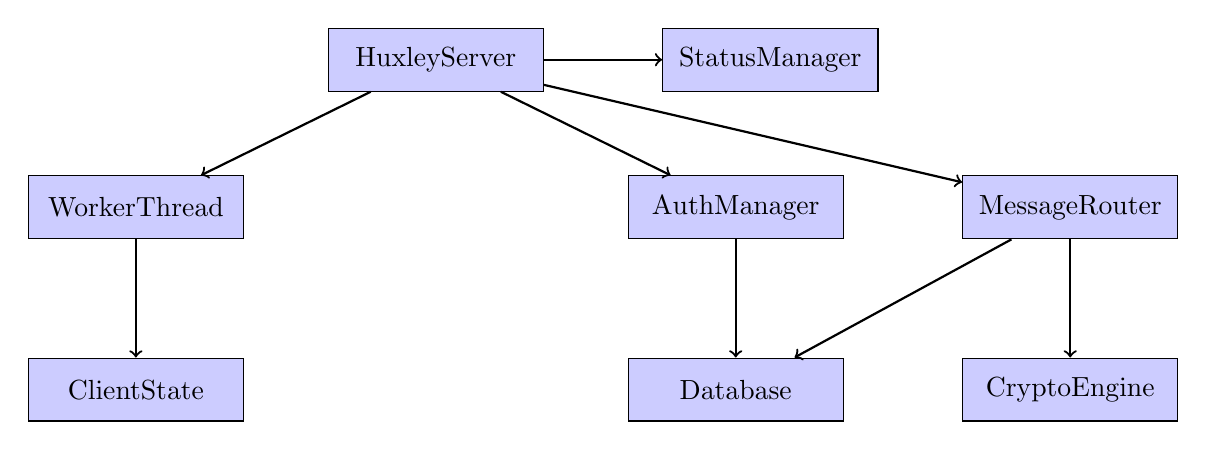
\begin{tikzpicture}[
            node distance=1.5cm,
            component/.style={rectangle, draw, fill=blue!20, text width=2.5cm, text centered, minimum height=0.8cm},
            arrow/.style={->, thick}
        ]
            % Main components
            \node[component] (server) {HuxleyServer};
            \node[component, below left=of server] (worker) {WorkerThread};
            \node[component, below=of worker] (client) {ClientState};
            \node[component, below right=of server] (auth) {AuthManager};
            \node[component, right=of auth] (router) {MessageRouter};
            \node[component, below=of auth] (db) {Database};
            \node[component, below=of router] (crypto) {CryptoEngine};
            \node[component, right=of server] (status) {StatusManager};
            
            % Arrows
            \draw[arrow] (server) -- (worker);
            \draw[arrow] (server) -- (auth);
            \draw[arrow] (server) -- (router);
            \draw[arrow] (server) -- (status);
            \draw[arrow] (worker) -- (client);
            \draw[arrow] (auth) -- (db);
            \draw[arrow] (router) -- (db);
            \draw[arrow] (router) -- (crypto);
        \end{tikzpicture}
    \end{center}
    
    \vspace{0.3cm}
    \textbf{Key Design Principles:}
    \begin{itemize}
        \item Clear separation of concerns
        \item Dependency injection for testability
        \item Abstraction over concrete implementations
    \end{itemize}
\end{frame}

\begin{frame}{Core Classes}
    \begin{columns}
        \column{0.5\textwidth}
        \textbf{HuxleyServer}
        \begin{itemize}
            \item Main orchestrator
            \item Manages worker thread pool
            \item Owns shared subsystems
            \item Accept loop coordinator
        \end{itemize}
        
        \vspace{0.3cm}
        \textbf{WorkerThread}
        \begin{itemize}
            \item Event-driven I/O multiplexing
            \item Private epoll instance
            \item Handles multiple clients
            \item Command dispatching
        \end{itemize}
        
        \vspace{0.3cm}
        \textbf{ClientState}
        \begin{itemize}
            \item Per-connection session state
            \item Authentication tracking
            \item I/O buffer management
            \item Send/receive queues
        \end{itemize}
        
        \column{0.5\textwidth}
        \textbf{AuthManager}
        \begin{itemize}
            \item User registration
            \item Credential verification
            \item Password hashing
            \item Database integration
        \end{itemize}
        
        \vspace{0.3cm}
        \textbf{MessageRouter}
        \begin{itemize}
            \item Message delivery logic
            \item Online/offline routing
            \item activeClients map
            \item Queue management
        \end{itemize}
        
        \vspace{0.3cm}
        \textbf{Database}
        \begin{itemize}
            \item SQLite interface
            \item Prepared statements
            \item WAL mode operations
            \item Transaction management
        \end{itemize}
    \end{columns}
\end{frame}

%===========================================
\section{Concurrency Design}
%===========================================

\begin{frame}{Thread Architecture}
    \begin{block}{Main Thread (Acceptor)}
        \begin{itemize}
            \item Single producer of client sockets
            \item Bootstraps subsystems
            \item Accept loop: \texttt{accept4()} → select worker → enqueue
            \item Least-loaded worker selection
        \end{itemize}
    \end{block}
    
    \begin{block}{Worker Threads (I/O Reactors)}
        \begin{itemize}
            \item Fixed-size pool (one per CPU core)
            \item Private \texttt{epoll} instance per worker
            \item Exclusive socket ownership
            \item Non-blocking I/O only
            \item Per-worker SQLite connection (WAL mode)
        \end{itemize}
    \end{block}
    
    \begin{alertblock}{Key Invariants}
        \begin{itemize}
            \item Exclusive socket ownership after assignment
            \item No socket shared across workers
            \item One DB handle per worker
        \end{itemize}
    \end{alertblock}
\end{frame}

\begin{frame}[fragile]{Worker Dispatcher Loop}
\begin{lstlisting}[language=C]
// Worker thread main loop
for (;;) {
    int n = epoll_wait(epollFd, events, MAX_EVENTS, 5000);
    
    if (n == 0) { 
        housekeeping();  // Timeouts, backpressure
        continue; 
    }
    
    for (int i = 0; i < n; ++i) {
        int fd = events[i].data.fd;
        uint32_t ev = events[i].events;
        
        if (fd == wakeupFd && (ev & EPOLLIN)) {
            drain_wakeup(wakeupFd);
            drain_assignments();  // New clients from main thread
            continue;
        }
        
        if (ev & (EPOLLHUP | EPOLLERR)) { 
            close_fd(fd); 
            continue; 
        }
        
        if (ev & EPOLLIN)  handleReadEvent(fd);
        if (ev & EPOLLOUT) handleWriteEvent(fd);
    }
}
\end{lstlisting}
\end{frame}

\begin{frame}{Synchronization Strategy}
    \begin{block}{Where We Lock}
        \begin{itemize}
            \item \textbf{Assignment Queues:} MPSC (multi-producer, single-consumer)
            \item \textbf{MessageRouter.activeClients:} Protected by \texttt{clientsMutex}
            \item \textbf{Per-client State:} No locking (worker-owned)
        \end{itemize}
    \end{block}
    
    \begin{block}{Deadlock Avoidance}
        \begin{itemize}
            \item Lock order invariant: \texttt{clientsMutex} $\prec$ \texttt{ledMutex}
            \item Minimal critical sections (map operations only)
            \item Copy-out, unlock, then act pattern
            \item Never hold lock during I/O operations
        \end{itemize}
    \end{block}
    
    \begin{block}{Correctness Properties}
        \begin{itemize}
            \item \textbf{At-least-once delivery:} Persist before send, mark delivered after
            \item \textbf{Progress:} Events serviced within one dispatcher cycle
            \item \textbf{Isolation:} Slow client cannot stall others
        \end{itemize}
    \end{block}
\end{frame}

\begin{frame}{Session Management}
    \begin{columns}
        \column{0.5\textwidth}
        \textbf{Authentication Flow}
        \begin{enumerate}
            \item Client sends LOGIN command
            \item AuthManager validates credentials
            \item Store username in ClientState
            \item Register in activeClients map
            \item Flush queued messages
        \end{enumerate}
        
        \vspace{0.3cm}
        \textbf{Timeout Policy}
        \begin{itemize}
            \item Idle timeout: 1800s (30 min)
            \item Check frequency: 5s
            \item Immediate disconnect on detection
            \item Client notification before close
        \end{itemize}
        
        \column{0.5\textwidth}
        \textbf{Session Termination}
        \begin{itemize}
            \item Explicit logout
            \item Idle timeout
            \item Socket disconnect
            \item Server shutdown
        \end{itemize}
        
        \vspace{0.3cm}
        \textbf{Cleanup Actions}
        \begin{itemize}
            \item Unregister from activeClients
            \item Close socket
            \item Release buffers
            \item Log event
        \end{itemize}
    \end{columns}
\end{frame}

%===========================================
\section{State Machines}
%===========================================

\begin{frame}{Client Connection FSM}
    \begin{center}
        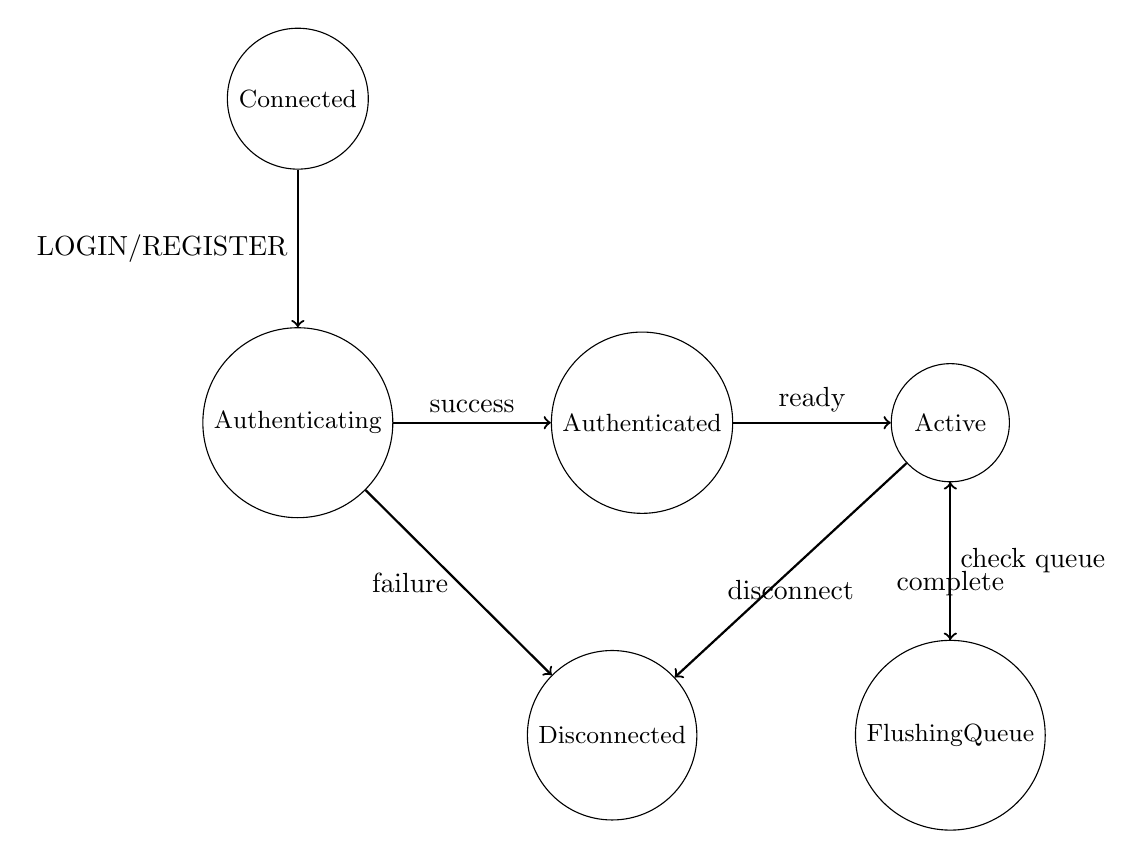
\begin{tikzpicture}[
            node distance=2cm,
            state/.style={circle, draw, minimum size=1.5cm, font=\small},
            arrow/.style={->, thick}
        ]
            \node[state] (connected) {Connected};
            \node[state, below=of connected] (auth) {Authenticating};
            \node[state, right=of auth] (authed) {Authenticated};
            \node[state, right=of authed] (active) {Active};
            \node[state, below=of active] (flush) {FlushingQueue};
            \node[state, left=of flush] (disc) {Disconnected};
            
            \draw[arrow] (connected) -- node[left] {LOGIN/REGISTER} (auth);
            \draw[arrow] (auth) -- node[above] {success} (authed);
            \draw[arrow] (auth) -- node[left] {failure} (disc);
            \draw[arrow] (authed) -- node[above] {ready} (active);
            \draw[arrow] (active) -- node[right] {check queue} (flush);
            \draw[arrow] (flush) -- node[below] {complete} (active);
            \draw[arrow] (active) -- node[below] {disconnect} (disc);
        \end{tikzpicture}
    \end{center}
    
    \textbf{Critical Transitions:}
    \begin{itemize}
        \item Authenticating → Authenticated: Register in activeClients map
        \item Authenticated → FlushingQueue: Query delivered=false messages
        \item Active → Disconnected: Cleanup and unregister
    \end{itemize}
\end{frame}

%===========================================
\section{Protocol Specification}
%===========================================

\begin{frame}[fragile]{Client-Server Protocol}
    \textbf{Frame Format:} Length-prefixed JSON over TCP
    \begin{center}
        \texttt{[4-byte length (network byte order)][JSON payload]}
    \end{center}
    
    \vspace{0.3cm}
    \begin{columns}
        \column{0.5\textwidth}
        \textbf{Sender (C)}
\begin{lstlisting}[language=C]
char json[] = 
  "{\"type\":\"LOGIN\","
  "\"username\":\"alice\","
  "\"password\":\"secret\"}";
uint32_t len = htonl(strlen(json));
send(sock, &len, sizeof(len), 0);
send(sock, json, strlen(json), 0);
\end{lstlisting}
        
        \column{0.5\textwidth}
        \textbf{Receiver (C)}
\begin{lstlisting}[language=C]
uint32_t len;
recv_all(sock, &len, sizeof(len));
len = ntohl(len);

char* buffer = malloc(len);
recv_all(sock, buffer, len);

// Parse JSON...
\end{lstlisting}
    \end{columns}
    
    \vspace{0.3cm}
    \begin{alertblock}{Why Length Prefix?}
        TCP is a byte stream - length prefix preserves message boundaries
    \end{alertblock}
\end{frame}

\begin{frame}[fragile]{JSON Message Examples}
    \begin{columns}
        \column{0.5\textwidth}
        \textbf{Registration}
\begin{lstlisting}[language=json]
{
  "type": "REGISTER",
  "username": "alice",
  "password": "secret123"
}
\end{lstlisting}

        \vspace{0.2cm}
        \textbf{Login}
\begin{lstlisting}[language=json]
{
  "type": "LOGIN",
  "username": "alice",
  "password": "secret123"
}
\end{lstlisting}

        \vspace{0.2cm}
        \textbf{Send Message}
\begin{lstlisting}[language=json]
{
  "type": "SEND_MESSAGE",
  "recipient": "bob",
  "content": "Hello Bob!"
}
\end{lstlisting}
        
        \column{0.5\textwidth}
        \textbf{Response}
\begin{lstlisting}[language=json]
{
  "type": "LOGIN_RESPONSE",
  "success": true
}
\end{lstlisting}

        \vspace{0.2cm}
        \textbf{Incoming Message}
\begin{lstlisting}[language=json]
{
  "type": "INCOMING_MESSAGE",
  "sender": "alice",
  "content": "Hello Bob!",
  "timestamp": "2025-01-15T14:30:00Z"
}
\end{lstlisting}

        \vspace{0.2cm}
        \textbf{Error}
\begin{lstlisting}[language=json]
{
  "type": "ERROR",
  "code": 401,
  "message": "Unauthorized"
}
\end{lstlisting}
    \end{columns}
\end{frame}

\begin{frame}{Error Codes}
    \begin{table}
        \centering
        \begin{tabular}{cl}
            \toprule
            \textbf{Code} & \textbf{Meaning} \\
            \midrule
            400 & Bad Request (malformed JSON/framing) \\
            401 & Unauthorized (invalid credentials) \\
            404 & Not Found (user does not exist) \\
            409 & Conflict (duplicate username) \\
            500 & Internal Server Error \\
            503 & Service Unavailable (server busy) \\
            \bottomrule
        \end{tabular}
    \end{table}
    
    \vspace{0.3cm}
    \begin{block}{Extensibility}
        Protocol is forward-compatible:
        \begin{itemize}
            \item Self-describing via \texttt{type} field
            \item Clients ignore unknown message types
            \item Can add features incrementally (group messaging, read receipts, presence)
        \end{itemize}
    \end{block}
\end{frame}

%===========================================
\section{Test Strategy}
%===========================================

\begin{frame}{Test Categories}
    \begin{columns}
        \column{0.5\textwidth}
        \textbf{Unit Tests}
        \begin{itemize}
            \item AuthManager: duplicate username rejection
            \item MessageRouter: online vs offline routing
            \item Database: prepared statement correctness
            \item CryptoEngine: encrypt/decrypt roundtrip
        \end{itemize}
        
        \vspace{0.3cm}
        \textbf{Integration Tests}
        \begin{itemize}
            \item End-to-end message delivery
            \item Login → send → receive → logout
            \item Memory leak detection (valgrind)
        \end{itemize}
        
        \column{0.5\textwidth}
        \textbf{Concurrency Tests}
        \begin{itemize}
            \item 25 simultaneous logins
            \item activeClients map thread safety
            \item SQLite WAL concurrent access
            \item Race condition detection (helgrind)
        \end{itemize}
        
        \vspace{0.3cm}
        \textbf{Security Tests}
        \begin{itemize}
            \item SQL injection attempts
            \item Brute force password testing
            \item Message tampering detection
            \item Timing attack resistance
        \end{itemize}
    \end{columns}
\end{frame}

\begin{frame}{Concurrency Test Example}
    \textbf{Test: ActiveClients Map Safety}
    
    \begin{block}{Setup}
        \begin{itemize}
            \item Thread 1: \texttt{unregisterClient("alice")}
            \item Thread 2: \texttt{unregisterClient("bob")}
            \item Run both 10,000 times concurrently
        \end{itemize}
    \end{block}
    
    \begin{block}{Verification}
        \begin{itemize}
            \item No segmentation faults
            \item No deadlocks
            \item No memory leaks
            \item Tool: \texttt{valgrind --tool=helgrind}
        \end{itemize}
    \end{block}
    
    \vspace{0.3cm}
    \textbf{Test: 25 Concurrent Logins}
    \begin{itemize}
        \item Pre-register 25 users
        \item Spawn 25 client threads
        \item Login simultaneously
        \item Expected: All succeed within 2 seconds
    \end{itemize}
\end{frame}

\begin{frame}{Security Test Example}
    \textbf{Test: SQL Injection}
    
    \begin{block}{Attack}
        Send username: \texttt{admin'; DROP TABLE users; --}
    \end{block}
    
    \begin{block}{Expected Behavior}
        \begin{itemize}
            \item Username stored as literal string
            \item Database tables remain intact
            \item No SQL execution from user input
        \end{itemize}
    \end{block}
    
    \vspace{0.3cm}
    \textbf{Test: Password Brute Force}
    \begin{itemize}
        \item Attempt 1000 password guesses
        \item Measure throughput
        \item Expected: <50 guesses/sec on RPi4
        \item Argon2id work factor prevents rapid testing
    \end{itemize}
\end{frame}

%===========================================
\section{Error Handling}
%===========================================

\begin{frame}{Error Classification}
    \begin{table}
        \centering
        \small
        \begin{tabular}{lll}
            \toprule
            \textbf{Level} & \textbf{Example} & \textbf{Action} \\
            \midrule
            CRITICAL & Port bind failure & Shutdown, retry with backoff \\
            ERROR & Database timeout & Notify client, log event \\
            WARNING & High memory usage & Alert admin, continue \\
            INFO & User login & Record for audit \\
            \bottomrule
        \end{tabular}
    \end{table}
    
    \vspace{0.3cm}
    \begin{block}{Recovery Mechanisms}
        \begin{itemize}
            \item \textbf{Database lock (SQLITE\_BUSY):} Exponential backoff, max 10 retries
            \item \textbf{Worker thread crash:} Watchdog detects, restart worker
            \item \textbf{Client disconnect:} Cleanup state, unregister, close socket
            \item \textbf{Memory exhaustion:} Reject new connections (503)
        \end{itemize}
    \end{block}
\end{frame}

\begin{frame}{Logging Strategy}
    \begin{columns}
        \column{0.5\textwidth}
        \textbf{Log Levels}
        \begin{itemize}
            \item DEBUG: Thread processing details
            \item INFO: User login/logout
            \item WARNING: Failed login attempts
            \item ERROR: Database failures
            \item CRITICAL: System shutdown
        \end{itemize}
        
        \vspace{0.3cm}
        \textbf{Examples}
        \begin{itemize}
            \item \texttt{INFO: User alice logged in}
            \item \texttt{WARNING: Failed login for eve (3rd attempt)}
            \item \texttt{ERROR: DB query failed after 10 retries}
        \end{itemize}
        
        \column{0.5\textwidth}
        \textbf{Rotation Policy}
        \begin{itemize}
            \item Mitigates microSD wear
            \item Prune when >10,000 entries
            \item Keep latest 5,000 logs
            \item Can offload to external syslog
        \end{itemize}
        
        \vspace{0.3cm}
        \textbf{Security Benefits}
        \begin{itemize}
            \item Audit trail for compliance
            \item Intrusion detection
            \item Failed login monitoring
            \item Debugging support
        \end{itemize}
    \end{columns}
\end{frame}

%===========================================
\section{Client Application}
%===========================================

\begin{frame}{Minimal CLI Client}
    \begin{columns}
        \column{0.5\textwidth}
        \textbf{Architecture}
        \begin{itemize}
            \item Three-layer design
            \item Main Loop: stdin/stdout
            \item MessageClient: high-level API
            \item ProtocolClient: socket wrapper
        \end{itemize}
        
        \vspace{0.3cm}
        \textbf{Technology}
        \begin{itemize}
            \item Python 3.x
            \item Built-in JSON support
            \item Standard library only
            \item ~200 lines of code
        \end{itemize}
        
        \column{0.5\textwidth}
        \textbf{Commands}
        \begin{itemize}
            \item \texttt{/register <user> <pw>}
            \item \texttt{/login <user> <pw>}
            \item \texttt{/send <recipient> <msg>}
            \item \texttt{/logout}
            \item \texttt{/quit}
        \end{itemize}
        
        \vspace{0.3cm}
        \textbf{Usage}
\begin{verbatim}
$ python client.py localhost 8080
> /register alice secret123
[SUCCESS] User registered
> /login alice secret123
[SUCCESS] Logged in as alice
> /send bob Hello!
[SUCCESS] Message sent
\end{verbatim}
    \end{columns}
\end{frame}

\begin{frame}{Client Design Rationale}
    \begin{block}{Why CLI over GUI?}
        \begin{itemize}
            \item Faster implementation (3 hours vs 2 days)
            \item Easier debugging
            \item Focuses on protocol correctness
            \item Testing tool for server development
        \end{itemize}
    \end{block}
    
    \begin{block}{Why Python?}
        \begin{itemize}
            \item Rapid prototyping
            \item JSON parsing built-in
            \item Cross-platform compatibility
            \item Reference implementation for third-party developers
        \end{itemize}
    \end{block}
    
    \begin{block}{Testing Role}
        \begin{itemize}
            \item Run multiple instances for concurrency testing
            \item Validate synchronization under load
            \item Attempt malformed inputs for security testing
            \item End-to-end flow verification
        \end{itemize}
    \end{block}
\end{frame}

%===========================================
\section{Sequence Diagrams}
%===========================================

\begin{frame}{User Registration Sequence}
    \begin{center}
        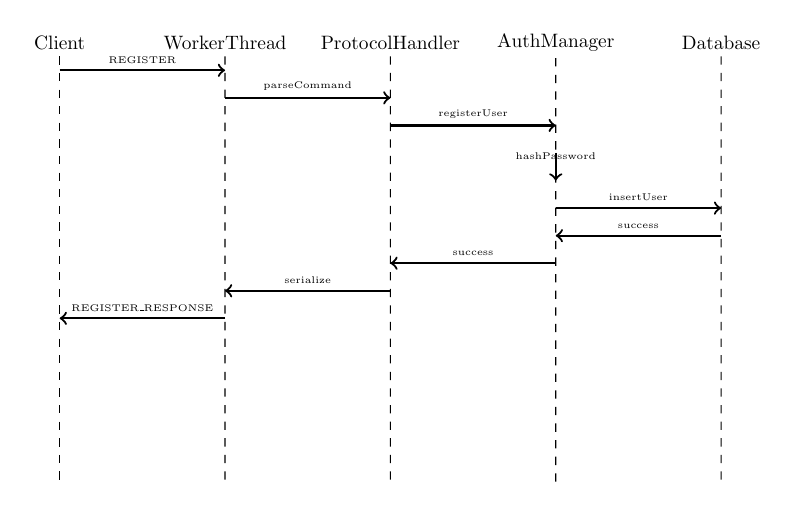
\begin{tikzpicture}[scale=0.7, transform shape]
            % Actors
            \node (client) at (0,0) {Client};
            \node (worker) at (3,0) {WorkerThread};
            \node (proto) at (6,0) {ProtocolHandler};
            \node (auth) at (9,0) {AuthManager};
            \node (db) at (12,0) {Database};
            
            % Lifelines
            \draw[dashed] (client) -- (0,-8);
            \draw[dashed] (worker) -- (3,-8);
            \draw[dashed] (proto) -- (6,-8);
            \draw[dashed] (auth) -- (9,-8);
            \draw[dashed] (db) -- (12,-8);
            
            % Messages
            \draw[->, thick] (0,-0.5) -- node[above] {\tiny REGISTER} (3,-0.5);
            \draw[->, thick] (3,-1) -- node[above] {\tiny parseCommand} (6,-1);
            \draw[->, thick] (6,-1.5) -- node[above] {\tiny registerUser} (9,-1.5);
            \draw[->, thick] (9,-2) -- node[above] {\tiny hashPassword} (9,-2.5);
            \draw[->, thick] (9,-3) -- node[above] {\tiny insertUser} (12,-3);
            \draw[->, thick] (12,-3.5) -- node[above] {\tiny success} (9,-3.5);
            \draw[->, thick] (9,-4) -- node[above] {\tiny success} (6,-4);
            \draw[->, thick] (6,-4.5) -- node[above] {\tiny serialize} (3,-4.5);
            \draw[->, thick] (3,-5) -- node[above] {\tiny REGISTER\_RESPONSE} (0,-5);
        \end{tikzpicture}
    \end{center}
\end{frame}

\begin{frame}{Message Send Sequence (Online Recipient)}
    \begin{center}
        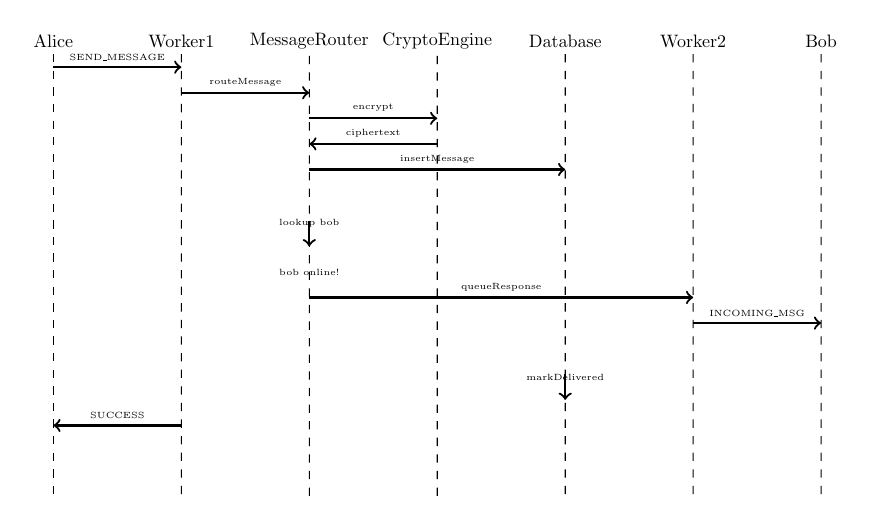
\begin{tikzpicture}[scale=0.65, transform shape]
            % Actors
            \node (alice) at (0,0) {Alice};
            \node (worker1) at (2.5,0) {Worker1};
            \node (router) at (5,0) {MessageRouter};
            \node (crypto) at (7.5,0) {CryptoEngine};
            \node (db) at (10,0) {Database};
            \node (worker2) at (12.5,0) {Worker2};
            \node (bob) at (15,0) {Bob};
            
            % Lifelines
            \draw[dashed] (alice) -- (0,-9);
            \draw[dashed] (worker1) -- (2.5,-9);
            \draw[dashed] (router) -- (5,-9);
            \draw[dashed] (crypto) -- (7.5,-9);
            \draw[dashed] (db) -- (10,-9);
            \draw[dashed] (worker2) -- (12.5,-9);
            \draw[dashed] (bob) -- (15,-9);
            
            % Messages
            \draw[->, thick] (0,-0.5) -- node[above] {\tiny SEND\_MESSAGE} (2.5,-0.5);
            \draw[->, thick] (2.5,-1) -- node[above] {\tiny routeMessage} (5,-1);
            \draw[->, thick] (5,-1.5) -- node[above] {\tiny encrypt} (7.5,-1.5);
            \draw[->, thick] (7.5,-2) -- node[above] {\tiny ciphertext} (5,-2);
            \draw[->, thick] (5,-2.5) -- node[above] {\tiny insertMessage} (10,-2.5);
            \draw[->, thick] (5,-3.5) -- node[above] {\tiny lookup bob} (5,-4);
            \node at (5,-4.5) {\tiny bob online!};
            \draw[->, thick] (5,-5) -- node[above] {\tiny queueResponse} (12.5,-5);
            \draw[->, thick] (12.5,-5.5) -- node[above] {\tiny INCOMING\_MSG} (15,-5.5);
            \draw[->, thick] (10,-6.5) -- node[above] {\tiny markDelivered} (10,-7);
            \draw[->, thick] (2.5,-7.5) -- node[above] {\tiny SUCCESS} (0,-7.5);
        \end{tikzpicture}
    \end{center}
\end{frame}

%===========================================
\section{Performance Considerations}
%===========================================

\begin{frame}{Performance Targets}
    \begin{columns}
        \column{0.5\textwidth}
        \textbf{Latency Requirements}
        \begin{itemize}
            \item Authentication: <1s
            \item Message send: <100ms
            \item Message delivery: <10ms (online)
            \item Queue flush: <500ms
        \end{itemize}
        
        \vspace{0.3cm}
        \textbf{Throughput Targets}
        \begin{itemize}
            \item 25+ concurrent users
            \item 100+ messages/second
            \item 1000+ messages/minute
        \end{itemize}
        
        \column{0.5\textwidth}
        \textbf{Resource Constraints}
        \begin{itemize}
            \item RAM: <512 MB
            \item CPU: 4 cores @ 1.5 GHz
            \item Storage: microSD (limited writes)
            \item Network: Gigabit Ethernet
        \end{itemize}
        
        \vspace{0.3cm}
        \textbf{Optimization Strategies}
        \begin{itemize}
            \item WAL mode for concurrency
            \item Prepared statement caching
            \item Fixed worker pool (no spawning)
            \item Bounded message queues
        \end{itemize}
    \end{columns}
\end{frame}

\begin{frame}{Scalability Analysis}
    \begin{block}{Current Design}
        \begin{itemize}
            \item 4 worker threads (one per core)
            \item Each worker handles ~6-7 clients
            \item Total: 25-28 concurrent connections
            \item Memory per client: ~16 KB (buffers + state)
        \end{itemize}
    \end{block}
    
    \begin{block}{Bottlenecks}
        \begin{itemize}
            \item \textbf{CPU:} Argon2id hashing (30ms per login)
            \item \textbf{I/O:} microSD write throughput
            \item \textbf{Memory:} Message queue depth × client count
            \item \textbf{Network:} TCP connection limits
        \end{itemize}
    \end{block}
    
    \begin{block}{Future Improvements}
        \begin{itemize}
            \item Redis for in-memory message queue
            \item PostgreSQL for production scale
            \item Load balancing across multiple RPi units
            \item Async I/O with io\_uring
        \end{itemize}
    \end{block}
\end{frame}

%===========================================
\section{Dry Run Example}
%===========================================

\begin{frame}[fragile]{Dry Run: Authentication Flow}
    \tiny
    \textbf{Scenario:} User "alice" logs in with password "secret123"
    
    \begin{tabular}{clp{3cm}p{6cm}}
        \toprule
        \textbf{Step} & \textbf{Thread} & \textbf{Function} & \textbf{Variables / Actions} \\
        \midrule
        1 & Worker 3 & handleReadEvent & buffer = \texttt{\{"type":"LOGIN",...\}} \\
        2 & Worker 3 & parseCommand & cmd.type=LOGIN, username="alice" \\
        3 & Worker 3 & processCommand & Dispatch LOGIN → AuthManager \\
        4 & Worker 3 & loginUser & username="alice", pw="secret123" \\
        5 & Worker 3 & findUser & SELECT password\_hash WHERE username=? \\
        6 & Worker 3 & sqlite3\_step & storedHash="\$argon2id\$..." \\
        7 & Worker 3 & verify & Compare hash vs password → success \\
        8 & Worker 3 & registerClient & lock(); activeClients["alice"]=state \\
        9 & Worker 3 & queueResponse & queue LOGIN\_RESPONSE, enable EPOLLOUT \\
        10 & Worker 3 & getQueuedMessages & SELECT WHERE delivered=0 \\
        11 & Worker 3 & sqlite3\_step & 3 undelivered messages found \\
        12 & Worker 3 & queueResponse & enqueue all messages to sendQueue \\
        13 & Worker 3 & handleWriteEvent & flush queue to socket \\
        \bottomrule
    \end{tabular}
    
    \vspace{0.2cm}
    \textbf{Total Time:} $\sim$50ms (dominated by Argon2id verification)
\end{frame}

%===========================================
\section{Conclusion}
%===========================================

\begin{frame}{Design Summary}
    \begin{block}{Architecture Highlights}
        \begin{itemize}
            \item Event-driven, multi-threaded server
            \item Fixed worker pool with epoll multiplexing
            \item SQLite WAL for concurrent database access
            \item Defense-in-depth security model
        \end{itemize}
    \end{block}
    
    \begin{block}{Key Innovations}
        \begin{itemize}
            \item Exclusive socket ownership eliminates locking overhead
            \item Length-prefixed JSON protocol ensures message boundaries
            \item At-least-once delivery with idempotent message IDs
            \item Per-worker SQLite connections maximize WAL concurrency
        \end{itemize}
    \end{block}
    
    \begin{block}{Security Guarantees}
        \begin{itemize}
            \item Memory-hard password hashing (Argon2id)
            \item Authenticated encryption (XSalsa20+Poly1305)
            \item SQL injection immunity (prepared statements)
            \item Comprehensive audit logging
        \end{itemize}
    \end{block}
\end{frame}

\begin{frame}{Design Validation}
    \begin{columns}
        \column{0.5\textwidth}
        \textbf{Correctness}
        \begin{itemize}
            \item Unit tests for each class
            \item Integration tests for workflows
            \item Concurrency tests (helgrind)
            \item Security penetration tests
        \end{itemize}
        
        \vspace{0.3cm}
        \textbf{Performance}
        \begin{itemize}
            \item Sub-second authentication
            \item 25+ concurrent connections
            \item <100ms message latency
            \item Bounded memory usage
        \end{itemize}
        
        \column{0.5\textwidth}
        \textbf{Maintainability}
        \begin{itemize}
            \item SOLID design principles
            \item Clear separation of concerns
            \item Comprehensive documentation
            \item Extensible protocol
        \end{itemize}
        
        \vspace{0.3cm}
        \textbf{Deployment}
        \begin{itemize}
            \item Embedded Linux (Buildroot)
            \item Cross-compilation toolchain
            \item Minimal resource footprint
            \item Production-ready security
        \end{itemize}
    \end{columns}
\end{frame}

\begin{frame}{Next Steps: Implementation Phase}
    \begin{enumerate}
        \item \textbf{Environment Setup}
        \begin{itemize}
            \item Configure Buildroot
            \item Set up cross-compilation
            \item Prepare development board
        \end{itemize}
        
        \item \textbf{Core Implementation}
        \begin{itemize}
            \item Database schema creation
            \item Thread pool and epoll dispatcher
            \item Protocol handler and command routing
        \end{itemize}
        
        \item \textbf{Security Integration}
        \begin{itemize}
            \item libsodium integration
            \item Password hashing and encryption
            \item Prepared statement implementation
        \end{itemize}
        
        \item \textbf{Testing \& Validation}
        \begin{itemize}
            \item Unit and integration tests
            \item Concurrency stress testing
            \item Security penetration testing
            \item Performance benchmarking
        \end{itemize}
    \end{enumerate}
\end{frame}

\begin{frame}{Future Enhancements}
    \begin{columns}
        \column{0.5\textwidth}
        \textbf{Protocol Extensions}
        \begin{itemize}
            \item Group messaging
            \item Read receipts
            \item Typing indicators
            \item User presence (online/offline)
            \item File transfer support
        \end{itemize}
        
        \vspace{0.3cm}
        \textbf{Security Enhancements}
        \begin{itemize}
            \item End-to-end encryption
            \item Per-user encryption keys
            \item Rate limiting (brute force)
            \item Two-factor authentication
        \end{itemize}
        
        \column{0.5\textwidth}
        \textbf{Performance Improvements}
        \begin{itemize}
            \item Redis message queue
            \item PostgreSQL backend
            \item Load balancing
            \item Connection pooling
        \end{itemize}
        
        \vspace{0.3cm}
        \textbf{Client Applications}
        \begin{itemize}
            \item GUI desktop client
            \item Mobile apps (iOS/Android)
            \item Web interface
            \item Third-party integrations
        \end{itemize}
    \end{columns}
\end{frame}

\begin{frame}[standout]
    \Huge Questions?
    
    \vspace{1cm}
    \normalsize
    \textbf{Huxley: Production-Ready Embedded Chat Server}
    
    \vspace{0.5cm}
    Secure • Scalable • Maintainable
\end{frame}

\begin{frame}{References}
    \small
    \begin{thebibliography}{99}
        \bibitem{argon2} \textit{Argon2: The Password Hashing Competition Winner}
        \\\url{https://github.com/P-H-C/phc-winner-argon2}
        
        \bibitem{libsodium} \textit{libsodium: Modern Cryptography Library}
        \\\url{https://libsodium.gitbook.io/}
        
        \bibitem{sqlite} \textit{SQLite: Write-Ahead Logging}
        \\\url{https://www.sqlite.org/wal.html}
        
        \bibitem{epoll} \textit{Linux epoll(7) Manual}
        \\\url{https://man7.org/linux/man-pages/man7/epoll.7.html}
        
        \bibitem{buildroot} \textit{Buildroot: Embedded Linux System}
        \\\url{https://buildroot.org/}
        
        \bibitem{rpi} \textit{Raspberry Pi 4 Documentation}
        \\\url{https://www.raspberrypi.com/documentation/}
    \end{thebibliography}
\end{frame}

\end{document}